% [Integrado desde drafts/ch7_conclusiones.tex el 2026-07-24. Pase 2.]
% Cierra la pregunta de investigación, los objetivos (ch1 sec:objetivos) y las brechas (sec:aporte).

\chapter{Conclusiones}
\label{ch:Conclusions}

Esta tesis se propuso comparar de forma sistemática tres estrategias de optimización
libres de gradiente, el algoritmo genético (GA), el híbrido con red neuronal sustituta
(NN+GA) y la optimización por enjambre de partículas (PSO), en el ajuste de los
parámetros de una cavidad láser ultrarrápida simulada, bajo idénticas condiciones y en
los regímenes de \emph{mode-locking} activo y pasivo. Realizado ese estudio comparativo
(Capítulo~\ref{ch:Results}), este capítulo responde la pregunta de investigación,
verifica el cumplimiento de los objetivos, recapitula las contribuciones y señala las
líneas de trabajo futuro.

\section{Respuesta a la pregunta de investigación}
\label{sec:conc_respuesta}

La pregunta que vertebró el trabajo era cómo se comparan el GA, el NN+GA y el PSO al
ajustar los parámetros de una cavidad láser ultrarrápida, evaluados bajo idénticas
condiciones de simulación y en ambos regímenes de anclaje, en cuanto a calidad del pulso,
costo computacional y robustez. % [REV-2026-11-17] ajustado a los controles de 2026-11 (drafts/originalidad/resultados_controles.md)
La respuesta es que, sobre la misma función de mérito, las tres estrategias alcanzan
soluciones factibles en todas sus corridas, pero difieren de manera medible en calidad,
eficiencia y comportamiento de búsqueda, de modo que el método preferible depende del
régimen.

En el régimen activo el PSO domina de forma inequívoca: alcanza el mayor valor de mérito
con diferencia estadísticamente significativa, la menor dispersión entre repeticiones, la
convergencia más rápida y, además, el óptimo más robusto. Su ventaja tiene una lectura
física: encuentra combinaciones de dispersión anómala y automodulación de fase que dan un
solitón más comprimido, y ninguna de sus corridas queda en la familia gaussiana de
Kuizenga--Siegman, donde terminan dos del GA y una del NN+GA. En el régimen pasivo, en cambio,
el PSO y el GA quedan estadísticamente empatados, sin ventaja apreciable de ninguno. El
sustituto neuronal iguala al GA en el régimen activo empleando $5{.}7$ veces menos
evaluaciones reales del simulador y pierde calidad en el pasivo, donde su mejor solución
ni siquiera es un óptimo local. Un control emparejado matiza ese ahorro: con setenta
evaluaciones, la red no se separa estadísticamente de su propio muestreo inicial, y en el
activo incluso un muestreo de setenta puntos sin optimización se acerca al GA. Bajo estos tres hallazgos late un único factor explicativo: la forma del
paisaje de optimización que cada régimen presenta a la búsqueda (más regular en el activo,
aunque con dos familias de soluciones, y multiestable y rugoso en el pasivo), que da cuenta a la vez del dominio del
PSO, del empate en el pasivo y del éxito desigual del sustituto. A ese cuadro se añade una
conclusión metodológica: la robustez local es una tercera dimensión de comparación que
discrimina entre métodos incluso cuando el valor de mérito los iguala, y que ningún estudio
centrado solo en la calidad del óptimo puede capturar.

\section{Cumplimiento de los objetivos}
\label{sec:conc_objetivos}

Los objetivos planteados en la Sección~\ref{sec:objetivos} se cumplieron en su totalidad.
Se implementó y validó un modelo numérico de la cavidad basado en la ecuación maestra de
Haus, que reproduce las soluciones analíticas conocidas (régimen activo de
Kuizenga--Siegman, absorbente saturable rápido y solitón disipativo) con acuerdos del
orden del $0.01\%$ al uno por ciento, y que sirvió como entorno de evaluación común
(objetivo primero). Sobre él se formuló el problema de optimización, con sus variables de
decisión, sus rangos y su restricción de estabilidad, y una función de mérito escalar
definida sobre los observables del pulso estacionario (objetivo segundo). Se implementaron
las tres estrategias: el GA como línea base, el NN+GA con una red sustituta acoplada para
reducir las evaluaciones costosas, y el PSO con su propia dinámica de enjambre (objetivos
tercero, cuarto y quinto). Finalmente, se enfrentaron los tres métodos en ambos regímenes
bajo un conjunto común de métricas (calidad, costo y robustez) manteniendo fijos el láser,
el espacio de parámetros y la función de mérito, de modo que las diferencias observadas se
atribuyen al algoritmo y no al problema (objetivo sexto), que constituye el aporte central
del trabajo.

\section{Contribuciones}
\label{sec:conc_contribuciones}

La contribución principal es un estudio comparativo controlado que ataca conjuntamente las
dos brechas identificadas en la Sección~\ref{sec:aporte}. Frente a la brecha de objeto (la
concentración de la optimización automatizada en el régimen pasivo), el trabajo extiende la
comparación al régimen activo y muestra que, lejos de ser más difícil, resulta el régimen
\emph{más} tratable para esta familia de metaheurísticas: su paisaje favorece la convergencia
rápida del PSO y permite que un muestreo de pocos puntos se acerque al GA, de modo que su menor presencia
en la literatura no obedece a una dificultad intrínseca de optimización sino, plausiblemente,
al menor interés aplicado de sus pulsos más largos. Frente a la brecha de método (los
estudios de caso aislados que impiden atribuir las diferencias al algoritmo), el diseño que
mantiene fijo todo salvo el optimizador es en sí mismo la contribución, pues permite afirmar
que la ventaja del PSO es una propiedad del método frente a un paisaje dado y no un
accidente del montaje.

De ese diseño se derivan aportes secundarios. El primero es un marco reproducible de
simulación y optimización (simulador validado, capa de problema con contabilidad exacta de
evaluaciones y los tres optimizadores) documentado con procedencia completa, sobre el que
pueden montarse comparaciones ulteriores. El segundo es un contraste del sustituto con su propio muestreo:
con setenta evaluaciones, su aporte no se separa estadísticamente del de un hipercubo
latino del mismo costo, una advertencia para cualquier estudio que atribuya a la red el
ahorro de un esquema NN+GA. El tercero es la evidencia de que los óptimos de mérito se
apoyan contra una frontera de factibilidad que se identificó en cada régimen (la ruptura
en multipulso en el pasivo y la pérdida del estado estacionario del solitón en el
activo), lo que convierte a la robustez en un criterio de selección de método tan
pertinente como la propia calidad.

\section{Relevancia y perspectivas}
\label{sec:conc_relevancia}

% [REV-2026-11-23b] SECCIÓN EN CONSTRUCCIÓN (observación 4 del director).
% Material movido literalmente desde el cap. 3 (§3.2.2: peine de frecuencias y CEO),
% que no se usaba en los caps. 4-5 pero es el puente físico hacia las aplicaciones.
% FALTA: conectar con espectroscopía de doble peine, bombeo-sonda, microscopía
% multifotónica y láseres autoajustables con ML; requiere pase 1 de la literatura.
% Sin sobrevender: el estudio es solo de simulación.
El tren de pulsos que se optimiza en esta tesis tiene, en el dominio espectral, la
estructura de un peine de frecuencias, y esa estructura es la que vincula el control de
la cavidad con las aplicaciones actuales de los láseres ultrarrápidos.

Conviene distinguir entre el espectro de un pulso aislado y el de un tren de pulsos. Un pulso único presenta un espectro continuo, mientras que la periodicidad del tren que impone la cavidad da un espectro discreto, o «peine de frecuencias». Como ilustra la Figura~\ref{fig:blockMode_CW}, el bloqueo de modos transforma una emisión multimodo incoherente (ruido) en una estructura localizada en el tiempo y muy estable.

\begin{figure}[h]
    \centering
    \begin{minipage}{0.47\textwidth}
        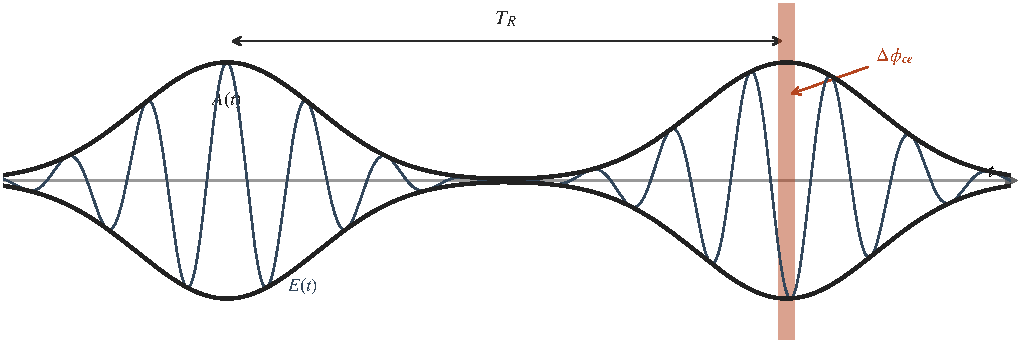
\includegraphics[width=\textwidth]{chapters/images/ch3/fig_ceo_time.pdf}\\
        \small (a) Dominio temporal.
    \end{minipage}
    \hfill
    \begin{minipage}{0.47\textwidth}
        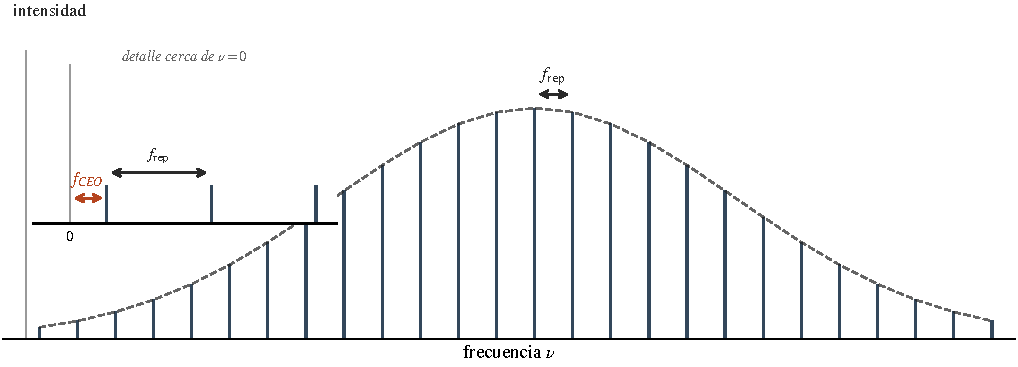
\includegraphics[width=\textwidth]{chapters/images/ch3/fig_comb.pdf}\\
        \small (b) Dominio espectral.
    \end{minipage}
    \caption[Dinámica temporal y espectral del tren de pulsos]{Dinámica temporal y espectral de un tren de pulsos ultracortos.
    (a) Dominio temporal, donde se ilustra la evolución de la fase
    portadora\-/envolvente (CEO). La disparidad entre las velocidades de grupo y de
    fase en la cavidad induce un desplazamiento relativo ($\Delta\phi_{ce}$) del
    campo eléctrico respecto a la envolvente en cada periodo de repetición $T_R$
    \cite{Keller2022}. (b) Dominio espectral, que evidencia la estructura de peine
    de frecuencias ópticas. El sistema posee dos grados de libertad fundamentales:
    el intervalo entre modos ($f_{\text{rep}} = 1/T_R$) y la frecuencia de
    compensación portadora\-/envolvente ($f_{CEO}$). En condiciones de dispersión
    nula, donde las velocidades de fase y de grupo coinciden, el campo eléctrico se
    reproduce idénticamente de pulso a pulso, resultando en un espectro cuyas
    líneas son múltiplos enteros de $f_{\text{rep}}$ ($f_{CEO}=0$)
    \cite{Keller2003}.}
    \label{fig:equidistantFrecuencyComb}
\end{figure}

En sistemas de pocos ciclos cobra importancia un grado de libertad crítico: el
desplazamiento de fase portadora\-/envolvente (\emph{carrier-envelope phase}, CEP).
Debido a la dispersión intracavidad, la velocidad de fase y la velocidad de grupo
difieren, provocando que el máximo del campo eléctrico se desplace respecto a la
envolvente del pulso en cada tránsito. Este fenómeno se traduce en el dominio
espectral como un desplazamiento global del peine de frecuencias por una cantidad
denominada frecuencia de compensación portadora\-/envolvente, $f_{CEO}$. Así, la
frecuencia de cada diente del peine queda definida por
$f_m = m\,f_{\text{rep}} + f_{CEO}$, parámetro fundamental en metrología de frecuencias y óptica de campo fuerte
\cite[cap.~12]{Keller2022}.

\section{Líneas de trabajo futuro}
\label{sec:conc_futuro}

Las limitaciones reconocidas al cierre del Capítulo~\ref{ch:Results} señalan el camino de
la extensión. La más inmediata es la validación experimental: todo el estudio se realizó en
simulación, sobre un modelo idealizado que no incorpora el ruido, la deriva de parámetros ni
la latencia de medición de un montaje real, de modo que trasladar los hallazgos a un
oscilador físico (y comprobar si el PSO conserva su ventaja en el régimen activo cuando el
paisaje se vuelve ruidoso) es el siguiente paso natural para cerrar la brecha \emph{sim\-/to\-/real}
\cite{Zhao2020}. Una segunda línea es incorporar el aprendizaje por refuerzo profundo, que
esta tesis dejó deliberadamente fuera de su núcleo comparativo: su capacidad para navegar la
multiestabilidad mediante políticas sobre un proceso de decisión lo hace especialmente
prometedor justo en el régimen pasivo, donde las metaheurísticas sin memoria empatan y el
sustituto no llega a aprender el paisaje con setenta muestras \cite{Kokhanovskiy2024}.

Otras extensiones amplían el alcance sin cambiar de paradigma. Reformular la función de
mérito como un problema multiobjetivo expondría explícitamente los compromisos entre
duración, energía y estabilidad que la ponderación escalar resume en un solo número, y
entregaría un frente de Pareto en lugar de un único óptimo. Enriquecer la física del modelo
(un absorbente saturable lento con formación de solitón tipo SESAM, otras cavidades de
referencia, un espacio de parámetros de mayor dimensión) pondría a prueba la generalidad de
las conclusiones más allá del absorbente rápido ideal. Un calendario del sustituto más largo y más repeticiones permitirían medir con potencia
suficiente si la red aporta sobre su muestreo, y repetir la optimización con otros pesos,
con hiperparámetros ajustados y con una caja de rangos más amplia acotaría la
dependencia de los resultados respecto de esas elecciones. Y evaluar la robustez de forma global,
no solo como sensibilidad local en torno al óptimo, permitiría medir la resiliencia frente a
los saltos entre atractores que caracterizan a la cavidad multiestable, allí donde el peor
caso observado advierte que la mediana no basta como garantía.

Con ello, el círculo abierto en la introducción se cierra: el ajuste de un láser ultrarrápido,
planteado como un problema de optimización de caja negra, admite soluciones automáticas de
calidad comparable por vías distintas, y la elección informada entre ellas (qué método, a qué
costo y con qué robustez) depende, ante todo, de la física del régimen sobre el que se
optimiza.
